\chapter{Mapping of 90° Contact Angle Droplets}

This chapter reconstructs a charged droplet situated on an electrically negligible layer, with a 90$\degree$ contact angle. The process uncovers that the Crowdy map contains analytical solutions for droplets on a charged substrate along with interesting equipotential patterns.

\section{Boundary Equation Derivation}
\subsection{Proposing the Problem}
The term ``Electrowetting" refers to distinct scenarios, such as the two cases in Figure \ref{fig:ew_2cases}. This chapter addresses a charged droplet on an electrically negligible substrate, surrounded by air.
\begin{figure}[H]
    \centering
\adjustbox{frame=0.25pt,frame,margin=0.1pt,color=mycolor}{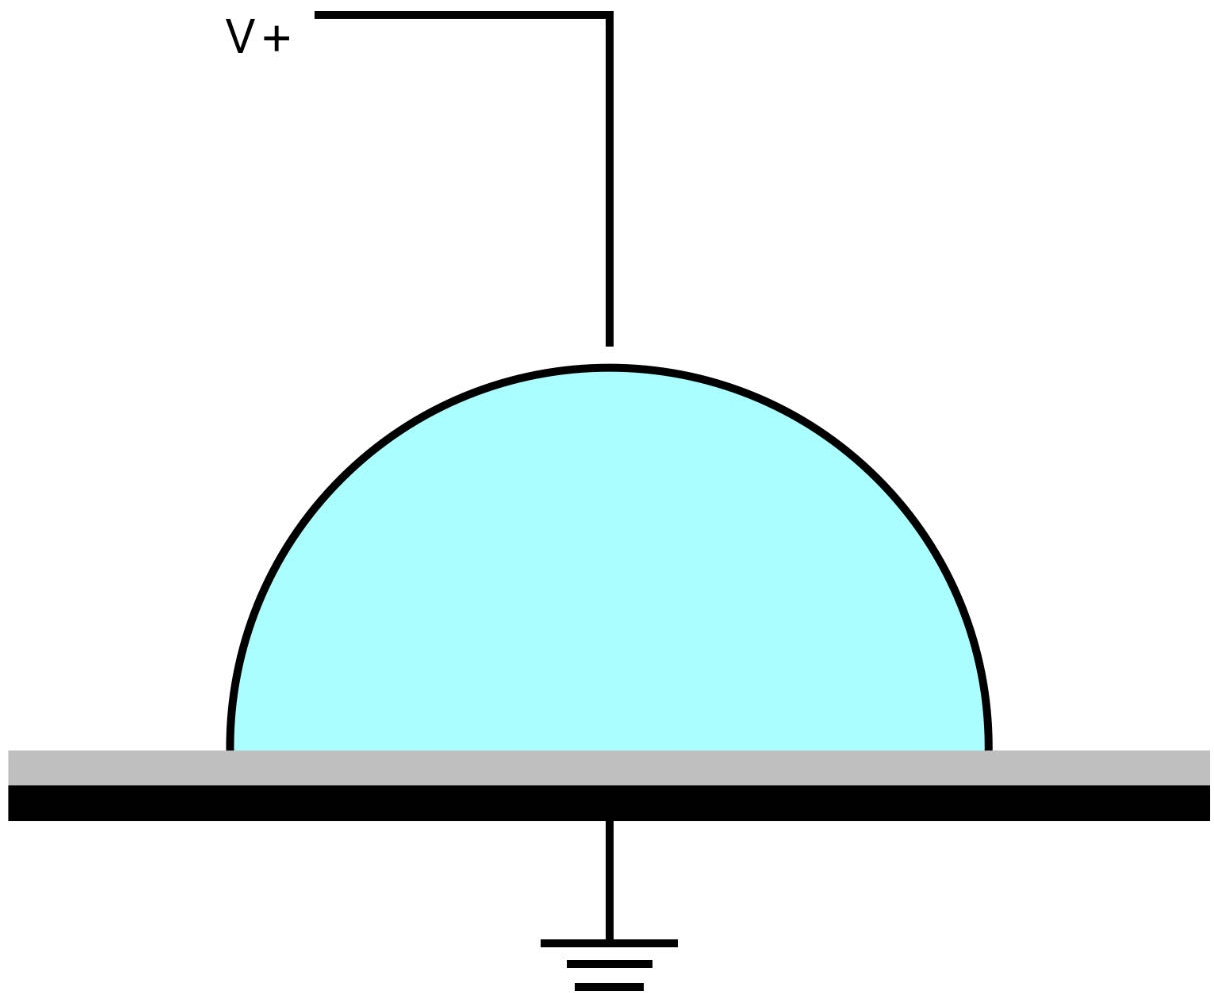
\includegraphics[width=0.405\linewidth]{Figs/sketch eletrode.jpg}}\hspace{.5em}
    \adjustbox{frame=0.25pt,frame,margin=0.1pt,color=mycolor}{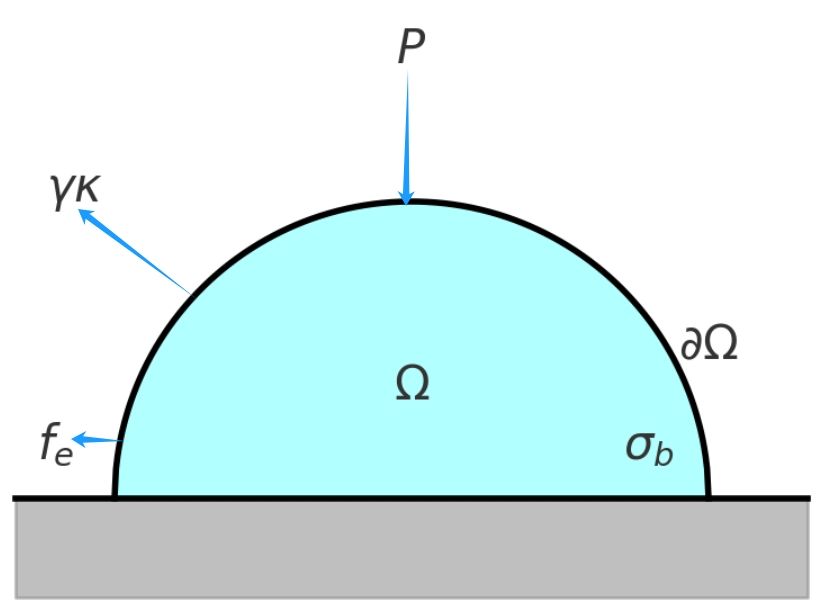
\includegraphics[width=0.445\linewidth]{Figs/setup, tension and force.png}} % Side by side images
    
    \caption{\small In the left figure, an electrode generates a voltage difference $V_+$ between the uncharged droplet and the conductor beneath an insulating layer. Meanwhile, the charged droplet with surface charge density $\sigma_b$ sits on an electrically negligible layer in the right figure. $\Omega\in\mathbb{R}^2$ represents the volume/area of the charged droplet. The balance between surface tension $\gamma\kappa$, pressure $P$, and the electric force $\vec{f}_e$—which is always a repulsive force—affects the droplet's shape $\partial \Omega$, while its volume $\Omega$ remains unchanged. The directions of $\gamma\kappa$ and $P$ depend on the specific conditions.
}
     \label{fig:ew_2cases}
\end{figure}
\noindent The conducting fluid droplet occupies $\Omega\in\mathbb{R}^2$ , the charge generates an electric field $\vec{E}$, together with the mechanical energy $\gamma\mathcal{P}$ from surface tension, the energy equation, which can date back to \citet{Rayleigh_1882}, is
\begin{equation}\label{eqn:minE}
    \mathcal{E} = \gamma \mathcal{P} - \frac{\epsilon_0 \epsilon_r}{2} \int_{R^2 \setminus \Omega} |E|^2 \, dS
\end{equation}

The electric energy $\mathcal{E}_e$ is the second term on the right of equation (\ref{eqn:minE}). The integral area ${\mathbb{R}^2 \setminus \Omega}$ implies that there is no electric field inside the droplet. $\epsilon_0 \epsilon_r$ is the permittivity, $\gamma$ is the surface tension, $\mathcal{P}$ is the length of the liquid-vapour interface, as defined in \citet{Crowdy2015}, equation (1).  The boundary equation on the liquid-vapour interface, from equation (\ref{eqn:minE}), is
\vspace{-0.5em}\begin{equation}\label{eqn:FonB}
\gamma \kappa - \frac{\sigma^2}{2 \epsilon_0 \epsilon_r} = -p\vspace{-0.5em}
\end{equation}
\subsection{Forces at the Stationary Boundary}
\hspace{0em}\indent \citet{Crowdy2015} proposed Equation (\ref{eqn:FonB}) by the variation of energy. Here, we first derive the equation (\ref{eqn:FonB}) from the forces on the droplet curve $\partial \Omega$. At any point on the droplet curve, let $\hat{n}$ be the normal direction pointing outward of the curve. The pressure difference $p\hat{n}$ and the surface tension, $\gamma \kappa \df l\hat{n} $, will be balanced by the electric force\footnote{Refer to equation (2.50), \citet{Griffiths_2017}, page 103.}
%\vspace{-0.5em}
\[
\vec{f}_e=\frac{\sigma}{2} (\vec{E}_{above}+\vec{E}_{below})%\vspace{-0.5em}
\]
The interior area of the conductor droplet is an equipotential area hence $\vec{E}_{below}\equiv0$, whereas  
%\vspace{-0.5em}
\[
\vec{E}_{above}|_{\partial \Omega}=-\nabla V|_{\partial \Omega}=-\left.\frac{\partial V}{\partial n}\hat{n}\right|_{\partial\Omega}%\vspace{-0.5em}
\]
$\vec{E}$ is caused by the surface charge density $\sigma$. According to equation (\ref{eqn:ed.line}) and equation (\ref{eqn:f.line}), the electrostatic pressure along the curve, is
%\vspace{-0.5em}
\[p_e=\frac{\sigma}{2}\left|\vec{E}_{above}\right|=-\frac{\sigma}{2}\frac{\partial V}{\partial n}=+\frac{\sigma^2}{2\epsilon_0\epsilon_r}%\vspace{-0.5em}
\]
This found the same result as in \citet{Fontelos2008}, equation (4). The force along $\hat{n}$ is:%\vspace{-0.75em}
\[0=\gamma\kappa\hat{n}+p\hat{n}+\frac{1}{2}\sigma \vec{E}%\vspace{-0.75em}
\]
In the stabilised circumstance, a charged conducting droplet has balanced electric force, pressure, and surface tension perpendicularly along its boundary line.
\subsection{Derivation Using the Divergence Theorem}
\hspace{0em}\indent We next try the divergence theorem. The variation in the electric field $\delta E_e$ is:
\begin{equation*}
    \delta \mathcal{E}_e=+\delta\left(-\frac{\epsilon}{2}\int_{\mathbb{R}^2\setminus\Omega}|E|^2 \df S
\right)=\int_{\delta\partial\Omega}...-\frac{\epsilon}{2}\int_{\mathbb{R}^2\setminus\Omega}\delta|E|^2 \df S\simeq-\frac{\epsilon}{2}\int_{\mathbb{R}^2\setminus\Omega}2\vec{E}\cdot\delta\vec{E} \df S
\end{equation*}
Let $\vec{G}\coloneqq\vec{E}\delta V$, $V$ is the voltage.
\begin{equation*}
    \begin{split}
    \delta \mathcal{E}_e&=-\epsilon\int_{\mathbb{R}^2\setminus\Omega}\vec{E}\cdot\delta(-\nabla V) \df S=\epsilon\int_{\mathbb{R}^2\setminus\Omega}\vec{E}\cdot(\nabla \delta V) \df S
    \end{split}
    \end{equation*}
Use $\nabla\cdot(\vec{A}\phi)=\phi\nabla\cdot\vec{A}+\vec{A}\cdot\nabla\phi$
\begin{equation}\label{eqn:div_find_0}
    \begin{split}
    \delta \mathcal{E}_e&=\epsilon\int_{\mathbb{R}^2\setminus\Omega}\nabla\cdot(\vec{E}\, \delta V) -\delta V \eqnmarkbox[black]{node1}{\nabla\cdot\vec{E}}\df S\\
    &=\epsilon\int_{\mathbb{R}^2\setminus\Omega}\nabla\cdot(\vec{E}\, \delta V) \df S \xlongequal[ ]{\text{div thm}}\oint_{...}\vec{G}\cdot\hat{n}\df l \epsilon=\int_{\partial \Omega}...+\eqnmarkbox[black]{node2}{\int_{r\rightarrow\infty}\vec{E}}\cdot\hat{n}\, \delta V\df l\\
    &=\epsilon\int_{\partial\Omega}\vec{E}\cdot\hat{n}\, \delta V \df l=\sigma\int_{\partial \Omega}\delta V \df l\\
    \end{split}
\end{equation}
\annotate[yshift=1em]{above, right, label above}{node1}{$\nabla \cdot \vec{E}|_{\mathbb{R}^2\setminus \Omega}= 0$}
\annotate[yshift=1em]{above, right, label above}{node2}{$=0,\vec{E}|_{r\rightarrow\infty}\rightarrow 0$}

\vspace{-1em}
\noindent Equation (\ref{eqn:ed.line}) shows $\vec{E}|_{\partial \Omega}=\sigma/\epsilon\hat{n}$. To have the desired result, we expect
\[\int_{\partial \Omega} \delta V \df l =-\frac{\sigma}{2\epsilon}\int_{\delta \partial \Omega}\df l\Longrightarrow\delta V = -\frac{\sigma}{2\epsilon}\delta l\]
Moreover\footnote{Refer to \cite{Griffiths_2017}, equation (2.50).}, \vspace{0.5em}
\[\delta V =  -\frac{1}{2}(\vec{E}_{above}+\eqnmarkbox[black]{node1}{{\vec{E}_{below}}})\cdot \delta \vec{l}=-\frac{\vec{E}_{above}}{2}\delta \vec{l}=-\frac{\sigma}{2\epsilon}\hat{n}\cdot \delta \vec{l}\]
\annotate[yshift=1.0em]{above, right, label above}{node1}{$=0$}

\vspace{-1.5em}
\noindent Since $V=\int \vec{E}\Longrightarrow \delta V \sim \vec{E}_{average}\cdot\delta\vec{d}$. Let $\delta l=\hat{n}\cdot\delta\vec{l}$, We derive the wanted equation,

\subsection{Variation of Minimal Energy Equation}
\label{Min_Eng}
\hspace{0em}\indent We lastly attempt the variation method. For energy minimization, a variation of the droplet curve $\delta\Omega$ leads to no change in energy, $\delta\mathcal{E}=0$. The corresponding variation in the surface tension and mechanical energy is:
\vspace{-0.5em}
\[\delta (\gamma\mathcal{P})=\gamma\delta\mathcal{P}\hspace{0.5em},\hspace{1em}\delta\mathcal{P}=\int_{\partial \delta\Omega}\kappa\df l\vspace{-0.5em}\]

Furthermore, since all the charges are distributed on the boundary $\partial \Omega$, assume\footnote{for a point charge, $E\sim r^{-2}\Longrightarrow\int E \sim O(r^{-1})$.} $\mathcal{E}_e|_{r\rightarrow\infty}\leq O(r^{-1})\sim 0$. Known $\mathcal{E}_e|_{\partial \Omega}=\sigma/\epsilon$ from equation (\ref{eqn:ed.line}), where $\sigma$ is the line charge density,
\[
\mathcal{E}_e=-\frac{\epsilon}{2}\int_{\mathbb{R}^2\setminus \Omega}|E|^2\df S=-\frac{\epsilon}{2}\int_{\partial \Omega}|\frac{\sigma}{\epsilon}|^2\df l+ \text{others} \Longrightarrow\delta \mathcal{E}_e \approx-\frac{\sigma^2}{2\epsilon}\int_{\partial \delta\Omega}\df l+\delta\, \text{others}
\]
Presume that a small variation of the boundary curve has a negligible effect in the region other than $\partial \Omega$, hence $\delta\, \text{others}\equiv0$, which is hinted in equation (\ref{eqn:div_find_0}). Sum up the two parts gives
\vspace{-0.5em}\[
\gamma \int_{\partial \Omega} \kappa \df l - \frac{\sigma^2}{2\epsilon}\int_{\partial \Omega}=0\vspace{-0.5em}
\]
Together with equation (\ref{Delta_P}), $\Delta p = \gamma \kappa$, the surface tension and pressure balance each other in the absence of electric force, we achieve the wanted formula.
\subsection{Boundary Charge Density and Non-dimensionalization}
\hspace{0em}\indent We reformulate equation (\ref{eqn:FonB}) in terms of the complex potential and apply non-dimensionalization to the formula for subsequent analysis. Define the complex potential of the electric potential V be
$w=U+\im V$ , where $U=\overline{V}$. For the harmonic function $\df_z w=\partial_x U+\im \partial_x V$. Known $\partial_x  U = \partial_y V$, hence on $\partial\Omega$, where $\Vec{E}=E\hat{n}=\nabla\cdot V=\partial V/\partial \hat{n}$, therefore:
\vspace{-0.5em}
\begin{equation}\label{eqn:wz_sigma}
\left|\frac{\df w}{\df z}\right|^2=\left|\partial_x V+\im\partial_y V\right|^2=\left|\nabla\cdot V\cdot\hat{n}\right|^2=|E|^2=\frac{\sigma^2}{\epsilon^2}\vspace{-0.5em}    
\end{equation}

Thus, rewrite equation (\ref{eqn:FonB}) as a function of $w$
\vspace{-0.5em}
\begin{equation}\label{eqn:boundary_w}
\gamma \kappa - \frac{\epsilon}{2}\left|\frac{\df w}{\df z}\right|^2 = -p\vspace{-0.5em}  
\end{equation}

Apply non-dimensionalization:\vspace{-1.em}
% \\ $z\coloneqq L\widetilde{z}$, 
% $ \kappa \coloneqq \widetilde{\kappa} / L$, 
% $w\coloneqq\widetilde{w}\sqrt{\gamma L/\epsilon}$, 
% $p\coloneqq\Gamma\gamma/L$, 
\[z\coloneqq L\widetilde{z}\hspace{2em}\kappa \coloneqq \widetilde{\kappa} / L\hspace{2em}w\coloneqq\widetilde{w}\sqrt{\gamma L/\epsilon}\hspace{2em}p\coloneqq\Gamma\gamma/L\]

$L$, $\Gamma$ are constants. Thus, equation (\ref{eqn:boundary_w}) becomes\footnote{Our derivation found a factor of $\frac{1}{2}$ difference from \citet{Crowdy2015}, which arises due to the setting of the constants and, therefore, does not have any real physics influence.}
%\vspace{-1.em}
\begin{equation}\label{eqn:dim.bl}
\widetilde{\kappa}-\frac{1}{2}\left|\frac{\df \widetilde{w}}{\df \widetilde{z}}\right|^2=-\Gamma
\end{equation}
\vspace{-4em}
\section{The Crowdy Map: Study and Extension}
\vspace{-1em}
\subsection{The Crowdy Map}

\hspace{0em}\indent The conformal mapping proposed in \citet{Crowdy2015} for the fixed $90^\circ$ contact angle case is:\vspace{-.5em}
\begin{equation}\label{eqn:crowdy_map}
z = i A \left( \frac{1}{\zeta} + \frac{8\zeta}{\zeta^2 - a^2} \right) \vspace{-.5em}
\end{equation}
It maps the upper boundary of a unit disc, describing a point charge (or point vortex), to the upper droplet curves for different capillary coefficients $a$.

\citet{Crowdy1999} and \citet{Crowdy2000} established this function. \citet{Crowdy2015} discovered that electrowetting, which has an identical boundary function, equation (\ref{eqn:dim.bl}), as bubble deformations, implies that these two distinct physical phenomena share mathematical congruence.
\begin{figure}[H]
    \centering
    \adjustbox{frame=0.25pt,frame,margin=0.1pt,color=mycolor}{
    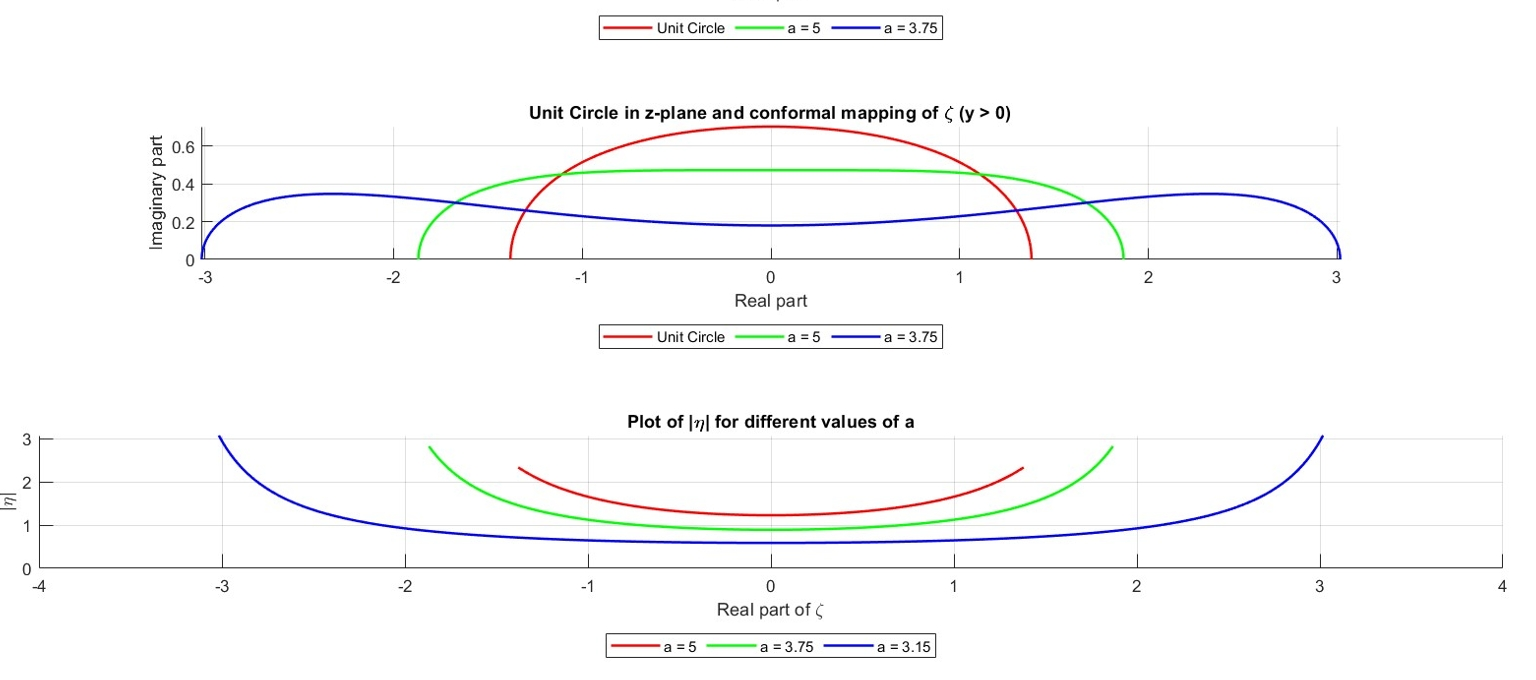
\includegraphics[width=1.\linewidth]{crowdy2015_re_cut.png}}
    \caption{\small Regenerated boundary shape and surface charge density of the charged droplets as described by Crowdy(2015), with different values of capillarity effort coefficients applied. The upper plot is the droplet shape, As \(a\) increases, two peaks near the ends of the droplet rise, while the middle part of the droplet lowers.  whereas in the lower plot of the surface charge densities, the "U"-shaped curve indicates that the charges accumulate at the two ends of the droplet's edge. A similar pattern was observed in \citet{Fontelos2008}.}
    \label{fig:enter-label}
\end{figure}

The correspondingly complex potential and surface charge density functions are\footnote{Refer to \ref{cpt:dev_w_e} for the derivation.}
\begin{equation}\label{eqn:crowdy.c}
    \begin{split}
        w &= W(\zeta) = i\mu \log \zeta\\
        \eta &= \left| \frac{dw}{dz} \right| = \left| \frac{W'(\zeta)}{Z'(\zeta)} \right| = \frac{\mu}{A} \left| \frac{\zeta^2 - a^2}{3\zeta^2 + a^2} \right|^2
    \end{split}
\end{equation}

 \subsection{The Feasibility of a Fixed Contact Angle}
\hspace{0em}\indent The mapping requires fixing the contact angle at $90\degree$. Simultaneously, the varying capillary coefficient $a$ will accumulate charges at the contact point, as shown in equation (\ref{eqn:crowdy.c}), hence affecting the curve shape there, as per equation (\ref{eqn:FonB}). This raises the question of whether the contact angle can remain fixed while both the surface charge density and the electric force increase.

Evidence from \citet{MugeleF2007} suggests that the contact angle does not change observably with charge accumulation. Numerical methods and physical observation show that the surface tension greatly exceeds the electric repulsive force at microscopic scales near the contact point. Consequently, the governing equation at the contact point is Young's equation (\ref{eqn:young}). However, at larger scales, the droplet’s surface curve bends further as charges gather, causing the contact angle measured at this scale to vary, and the droplet curve changes shape corresponding to equation (\ref{eqn:FonB}). This finding supports the feasibility of assuming an invariable contact angle in the mapping of a very small region in the study. 
\subsection{From Droplet's Curve to Its Potential: A Failed Attempt}
\hspace{0em}\indent The Crowdy map projects the unit circle to the shape below, which contains the upper droplet curve, that is, the contact line between the droplet and air above. The projected lines from the concentric circles on $\zeta$-plane represent the equipotentials of the charged bubble in Figure (\ref{fig:bubble_pot}). Since only part of the droplet's boundary is projected, They are not the voltages of the droplet in this study.
\begin{figure}[H]
    \centering
    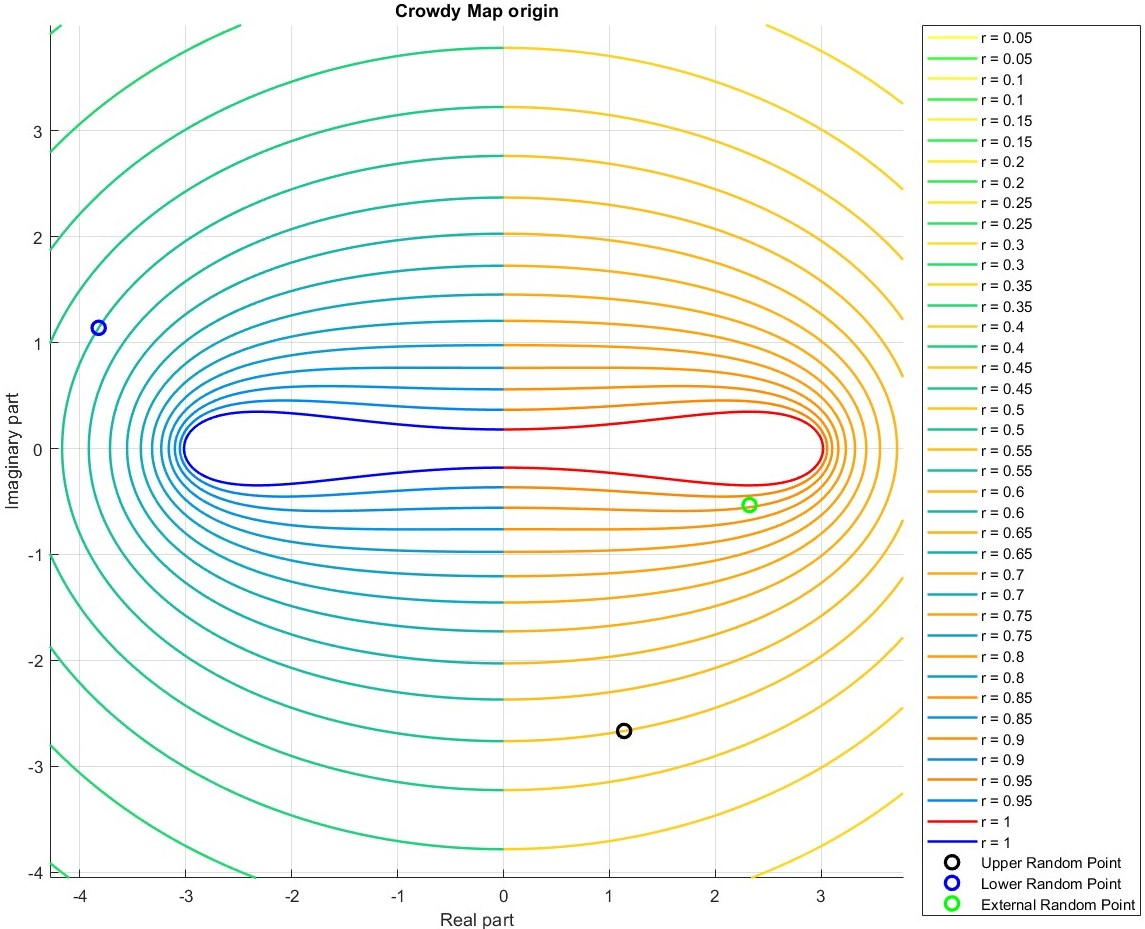
\includegraphics[width=1\linewidth]{Figs/crowdy 1-1.jpg}
    \caption{\small The Crowdy map projects the boundary of a unit circle on $\zeta$ onto the upper boundary of the droplet and its symmetric counterpart along the x-axis, forming the shape of a bubble. A brief exploration reveals that the arc from $-\pi/2$ to $\pi/2$ maps to the upper boundary, while the arc from $\pi/2$ to $3\pi/2$ maps to its mirror image along the x-axis. Furthermore, the closed curves surrounding the bubble, representing the bubble's equipotentials, corresponds to the concentric circles on $\zeta$ inside the unit circle.}
    \label{fig:bubble_pot}
\end{figure}
It is tempting to map the droplet's entire boundary to a unit circle on the $\zeta$-plane. Though this, the droplet's boundary, being an equipotential, is represented by the unit circle on $\zeta$, which corresponds to the equipotential of a point charge. Thus the droplet's complex potential can be determined, it would be simply the mapping of a point charge's complex potential.
% we can derive the complex potential based on the mapping. Therefore, the mapping essentially projects the geometry of a simple charge distribution to a complicated one. Applying the mapping to the simple potential function presents that of the more intricate charge distribution.

We want a closed curve from inside the unit circle on $\zeta$, via the Crowdy map, to the droplet's entire boundary. However, the $1/\zeta$ term in the mapping function (\ref{eqn:crowdy_map}) obstructs and the projection function diverges at the origin. To avoid this, we start with the inverse map. After some attempts, we found that a semi-circle, via a combination of the inverse map and the Crowdy map\footnote{Refer to \ref{cpt:boundary_map_fail} for details.}, presents the droplet's entire boundary exactly, as Figure (\ref{fig:droplet_entire_boundary}) shows.
\begin{figure}[h]
\centering
\adjustbox{frame=0.25pt,frame,margin=0.15,color=mycolor}{
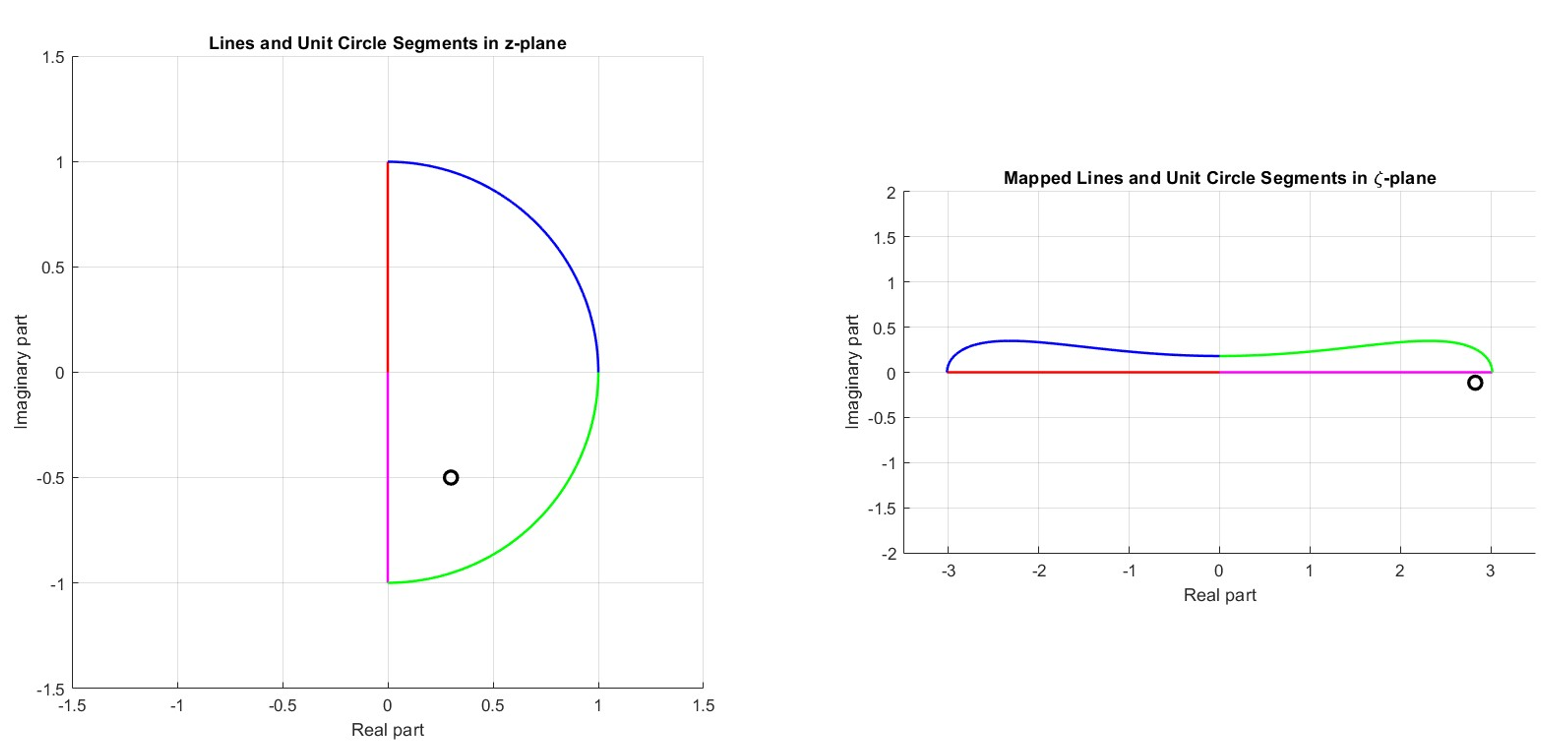
\includegraphics[width=1.\textwidth]{Figs/crowdy2015_edit.png}}
\caption{\small The closed semi-circle formed by the arc and the y-axis on the $\zeta$-plane is projected onto the droplet's entire boundary, including the contact line between the droplet and the substrate, via the inversed map followed by the Crowdy map. The four coloured lines in red, blue, green and purple, show how each part of the boundary is mapped. The circles in two plots show the inner area on $\zeta$ maps to the outer area on $z$, yet further investigation reveals that it is actually not a 1-1 mapping.}
\label{fig:droplet_entire_boundary}
\end{figure}

Achieving this, we expect that the complex potential for the droplet case could be derived from the mapping. Yet, the endeavour fails because the Crowdy map is a 1-1 projection only inside the unit circle on the $\zeta$-plane. 

When the inverse map is applied, the 1-1 property breaks, resulting in the crossing of projection lines on the $z$-plane, which were meant to be equipotentials that should not intersect, as Figure (\ref{fig:crowdy_inverse}) shows. Therefore, the combined mapping lacks physical meaning and cannot be the complex potential outside the charged droplet.

Furthermore, the origin of the $\zeta$-plane maps to infinity, and all points within the unit circle on the $\zeta$-plane are mapped to the exterior of the bubble. As a result, no line from the 1-1 region in the $\zeta$-plane is mapped to the lower droplet curve within the bubble's boundary. Consequently, the complex potential of the droplet appears unattainable  though this mapping. 
\begin{figure}[H]
    \centering
    \adjustbox{frame=0.25pt,frame,margin=0.15,color=mycolor}{
    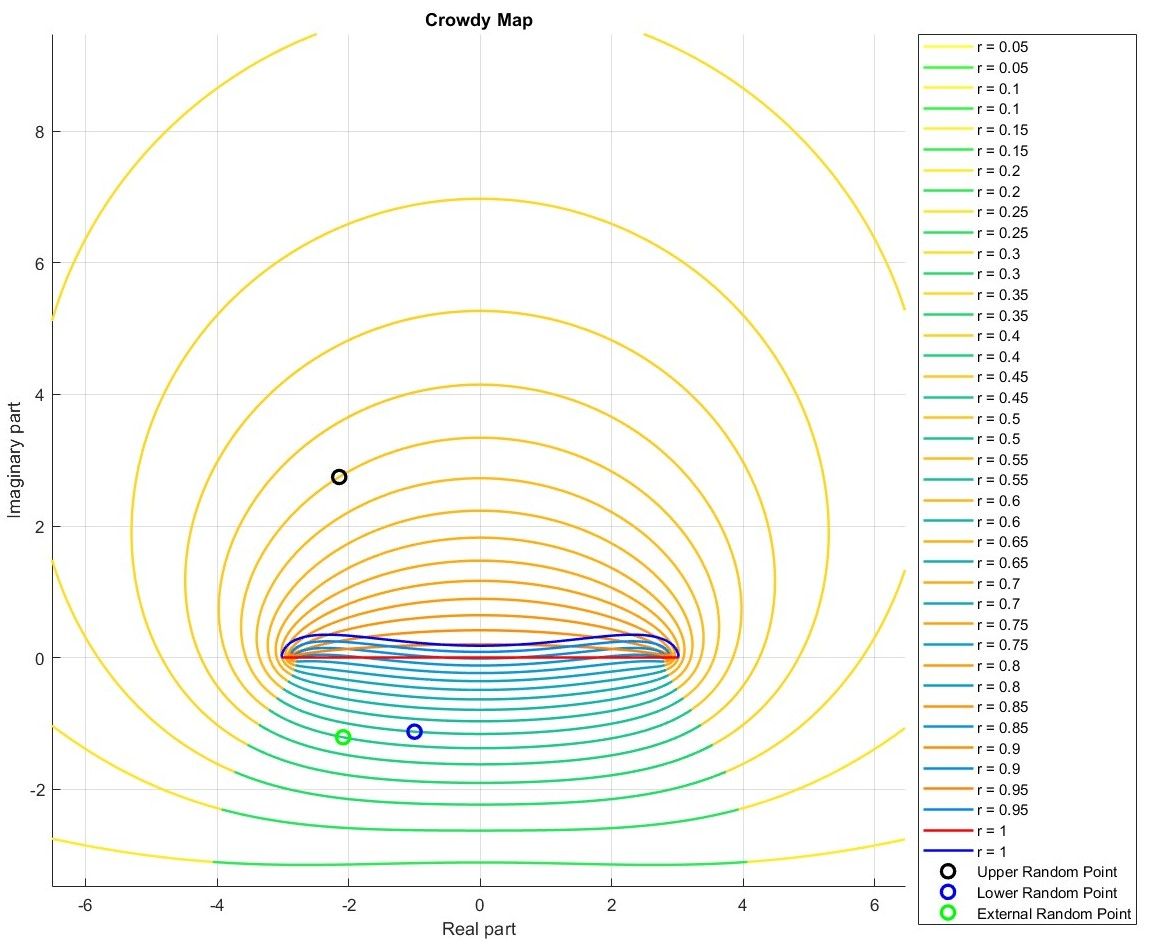
\includegraphics[width=1\linewidth]{Figs/crowdy inverse pot.jpg}}
    \caption{\small the projection lines on the $z$-plane come from the concentric circles on the $\zeta$-plane. Intersections are found along the droplet curve, implying that in the region where the concentric circles approach $r=1$ on $\zeta$, the mapping is not 1-1, and thus the has no clear physical meaning on $z$.}
    \label{fig:crowdy_inverse}
\end{figure}

\subsection{Extension of Crowdy Map: Droplets on Conducting Substrate}
\hspace{0em}\indent Though we fail to reach the droplet's potential, another physically reasonable complex potential within the Crowdy map is discovered. 
The potential is found by a combination of the semi-circle map and the Crowdy map, where the semi-circle map is\footnote{Refer to \ref{cpt:zeta_in_eta} for the inverse form and \ref{cpt:maps_combine} and \ref{cpt:hyper} for dteails.}:      
\begin{equation}\label{eqn:semi_map}
    \eta = \left(1 - \sqrt{\im\frac{1 - \zeta}{\zeta + 1}}\right)/\left(1 + \sqrt{\im\frac{1 - \zeta}{\zeta + 1}}\right) = \tanh \left( \frac{1}{2} \log \left( \frac{1+\im}{\sqrt{2}}\sqrt{\frac{1 - \zeta}{\zeta + 1} } \right) \right)
\end{equation}

The process is introduced here in parts:
\begin{enumerate}
    \item \textbf{Initial Setup}: On the $\zeta$-plane, concentric circles with radii ranging from 0.05 to 1 are generated, representing the inverse map of the equipotentials of a charged disc of radius 1.
    \begin{figure}[H]
        \centering
        \adjustbox{frame=0.25pt,frame,margin=0.15,color=mycolor}{
        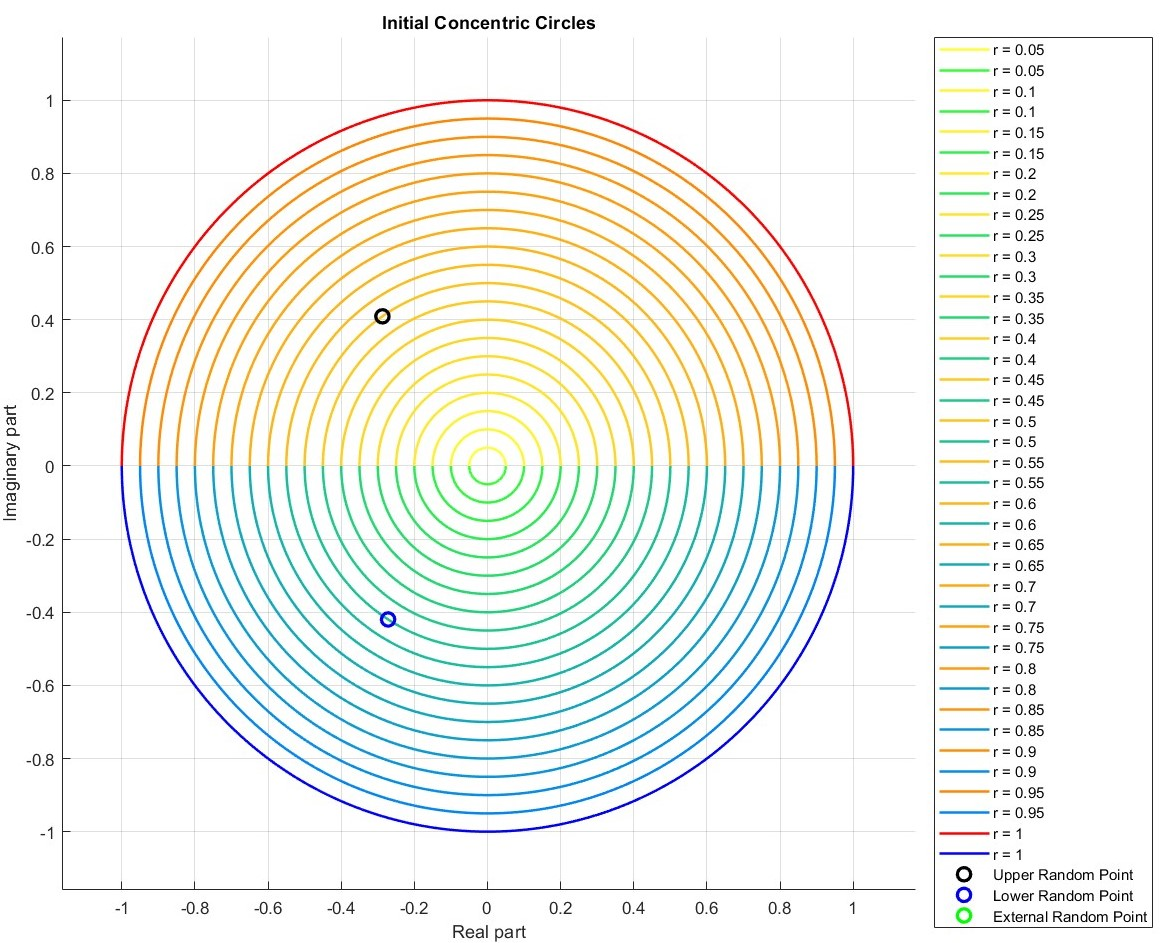
\includegraphics[width=1.\linewidth]
        {Figs/unit circle 1.jpg}}
        \caption{\small Concentric circles with radii correspond to colours. The upper circles use colours from yellow to red, while the lower circles use colours from green to blue. The three points in black, blue and green select coordinates from the upper area and lower area inside the unit circle, and somewhere outside, to check the following process.}
        \label{fig:enter-label}
        \end{figure}
    \item \textbf{The Cayley Map\footnote{Due to MATLAB's numerical limitations, the outermost circle's radius $r=1$ is adjusted to $(1 - 1 \times 10^{-15})$.}, followed by an rotation mapping}: Applies the transformation:\vspace{-1.em}
    \[
    \zeta_1 = \frac{1 - \zeta}{1 + \zeta}\vspace{-1.em}
    \]
    Multiplies the result by the imaginary unit:\vspace{-1.em}
    \[
    \zeta_2 = i \zeta_1
    \]
    \begin{figure}[H]
        \centering
        \adjustbox{frame=0.25pt,frame,margin=0.95,color=mycolor}{
        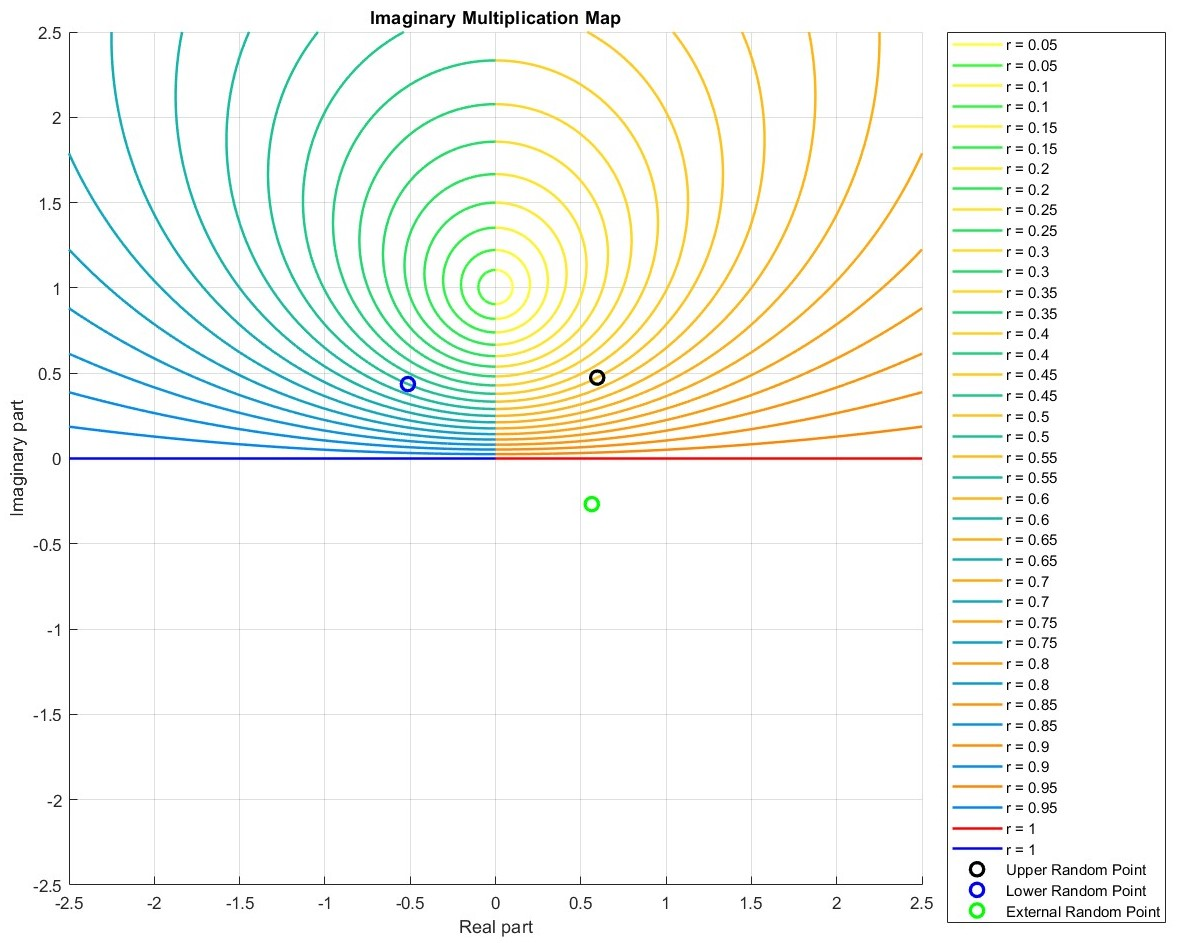
\includegraphics[width=1.\linewidth]{Figs/rot i.jpg}}
        \caption{\small The Cayley map, transforms the Concentric circles to the right half of the mapped $\zeta_1$-plane. Then, times $\im$, rotates the plots by $\pi/2$, to the upper half of $\zeta_2$-plane. The green point correctly maps to somewhere under the $x$-axis.}
        \label{fig:enter-label}
    \end{figure}
 
    \item \textbf{The square root mapping}: Applies a square root transformation, as Figure \ref{fig:sqrt} shows.
    \[
    \zeta_3 = \sqrt{\zeta_2}
    \]
    \item \textbf{Semi-Circle Map\footnote{In the programming, we replaced \(r=1\) upper half circle points with points along the y-axis from \(y=1\) to \(y=-1\), and lower half circle points with points from \(\theta = -\pi/2\) to \(\pi/2\), after this mapping.}}: Uses an inverse Cayley transformation, as Figure \ref{fig:semi-circle} shows.
    \[
    \eta = i \frac{1 - \zeta_3}{1 + \zeta_3}
    \]
    to map the first quadrant on $\zeta_3$ to the semi-circle on $\eta$
    \begin{figure}[H]
        \centering
        \adjustbox{frame=0.25pt,frame,margin=0.15,color=mycolor}{
        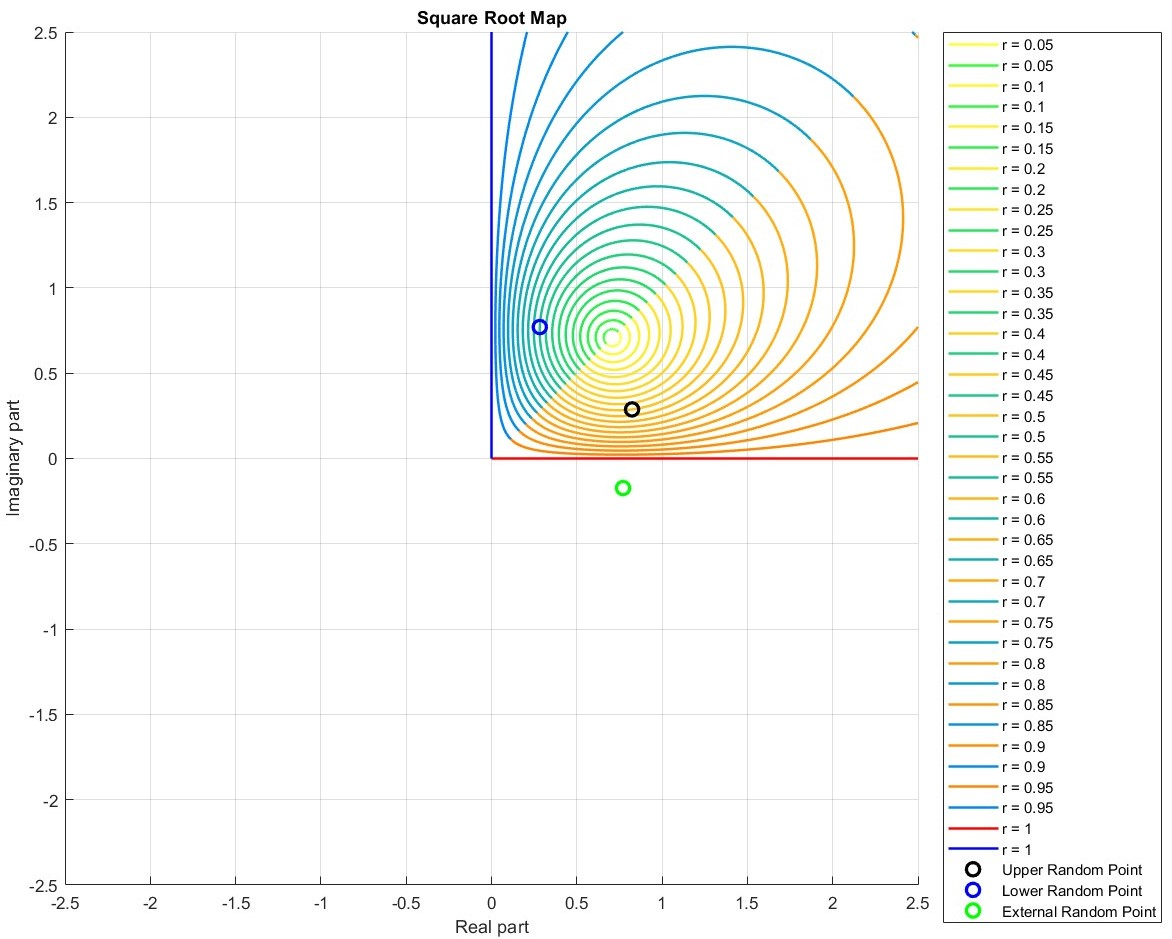
\includegraphics[width=.77\linewidth]{Figs/sqrt.jpg}}
        \caption{\small The square root transformation rotates the blue line, corresponding to $\theta=\pi$, to the $+y$-axis. From the green point, we observe that MATLAB selects a branch cut where the angle of the green point is interpreted as negative, rather than an angle close to $2\pi$.}
        \label{fig:sqrt}
    \end{figure}
    \begin{figure}[H]
        \centering    
        \adjustbox{frame=0.25pt,frame,margin=0.15,color=mycolor}{
        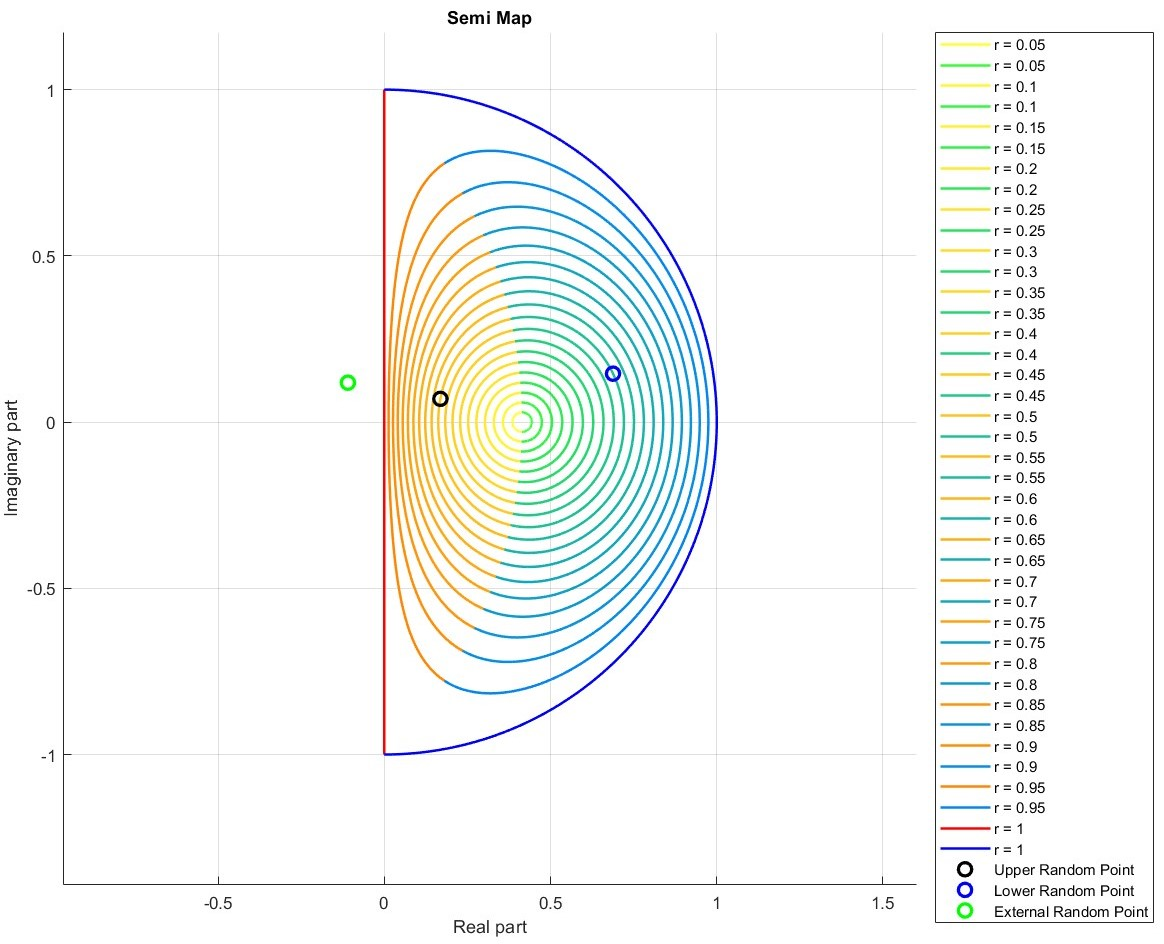
\includegraphics[width=.77\linewidth]{Figs/semi.jpg}}
        \caption{The inverse Cayley transformation map.}
        \label{fig:semi-circle}
    \end{figure}

 
   
    \item \textbf{Apple the Crowdy Map}: Applies the transformation:
    \begin{equation}\label{eqn:crowdy_eta}
        z = iA \frac{9\eta^2 - a^2}{\eta^3 - a^2 \eta}    
    \end{equation}
    where $a\geq3$ is the capillary coefficient, and $A=(a^4-1)/\sqrt{a^8-66a^4-63}$, as defined in \citet{Crowdy2015}. Figure \ref{fig:crowdy_f} shows the graph, with $a=3.15$ in the mapping.
    \end{enumerate}
        
    \begin{figure}[H]
    \centering    
    \adjustbox{frame=0.25pt,frame,margin=0.15,color=mycolor}{
    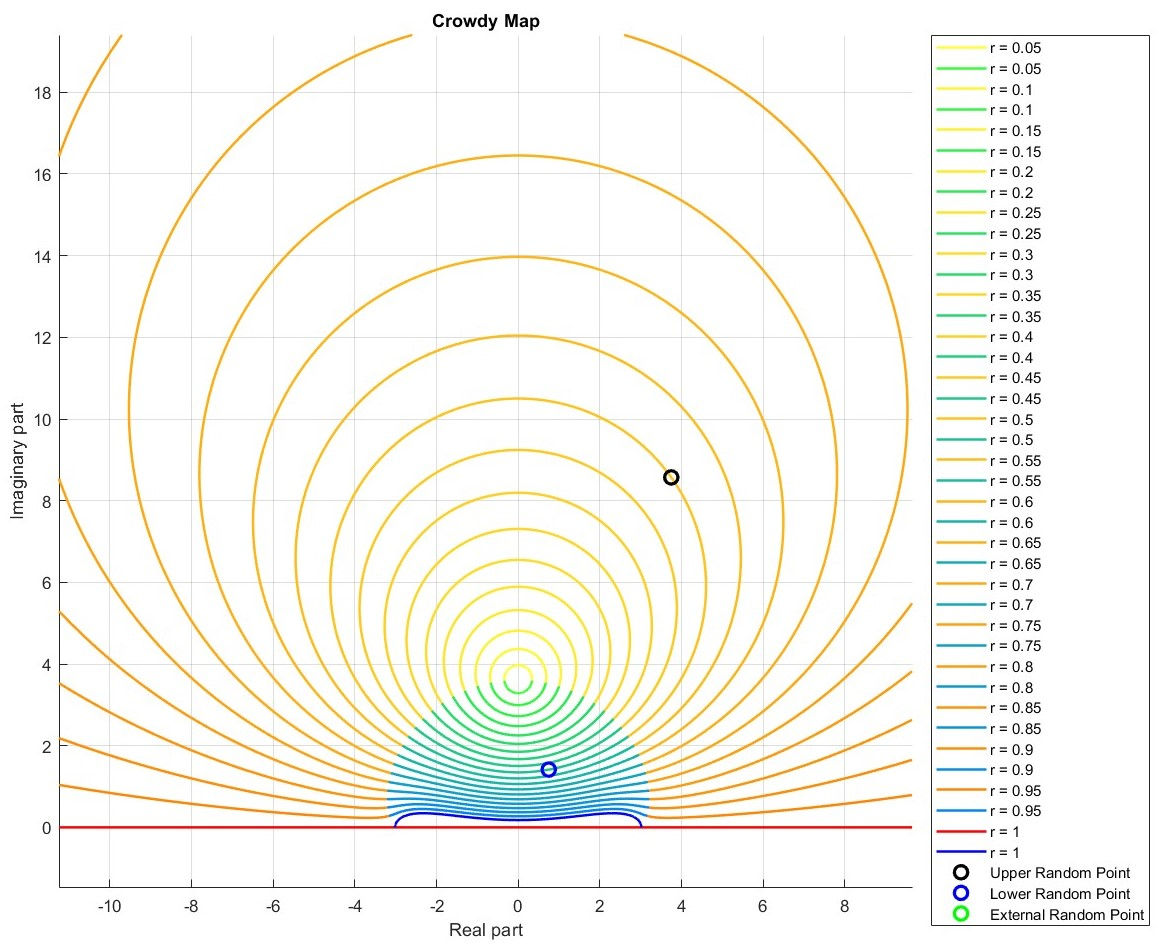
\includegraphics[width=1.\linewidth]{crowdy pot.jpg}}
    \caption{\small The Crowdy map of the closed curves in the semi-circle region in Figure \ref{fig:semi-circle}. The combination of mappings ultimately transforms the concentric circles inside a unit circle onto the pattern displayed above. The red line at $y=0$ is mapped from the upper curve of the unit circle on $\zeta$, whilst the blue line, representing the upper droplet curve, is mapped from the lower curve of the unit circle. The centre of the $\zeta$-plane is mapped to the circle above the droplet.
    } 
    \label{fig:crowdy_f}
\end{figure}

The complex potential is the combination of mapping (\ref{eqn:semi_map}), mapping (\ref{eqn:crowdy_eta}) and the complex potential of a point charge (\ref{eqn:crowdy.c}),
in the form $w(\zeta(z))$, although equation \ref{eqn:crowdy_eta} leads to a multivalued $\zeta(z)$. The exact form will not be given here.

The equipotentials of the mapping exhibit an interesting pattern. Each curve in Figure \ref{fig:crowdy_f} represents an equipotential of the charged disc on $\zeta$, hence the connected red line and blue line, which form the upper droplet curve and the boundary of the plate, respectively, constitute an equipotential, implies that both are conductors, with charge distributed along their shared boundary. Hence, the complex potential we have found corresponds to that of a conducting droplet above a conducting plate.

Whereas the other curves represent the equipotentials of the charge distribution, There is an induced point charge above the droplet. An infinitely long conducting plate would generate an electric field normal to the plate that extends to infinity, therefore, the induced charge is a result of the droplet's influence.

The location of the induced charge is a function of a. Since it comes from the origin on $\zeta$, which maps to 
\[\eta_0=\frac{1-\im}{1+\im}\]
according to the mapping equation (\ref{eqn:semi_map}), and then on the $z$-plane, the induced charge is located at
\[
z=\im A \frac{9\eta_0^2-a^2}{\eta_0^3-a^2\eta_0}
\]
according to the mapping equation (\ref{eqn:crowdy_eta}).

Moreover, the equipotentials in this scenario are somewhat analogous to the situation in fluid dynamics, where vortices can form when a fluid flows over a convex surface under certain conditions. For example, the aerodynamic shape of a racing car, which can be seen as a droplet in this context, may generate vortices\footnote{\href{https://www.explainthatstuff.com/aerodynamics.html}{Aerodynamics: an introduction}}.
 




\section{Summary}
This chapter discusses the boundary equation of a charged droplet with a 90$\degree$ contact angle. Using mechanical methods, the divergence theorem, and the variational method, the Bernoulli condition of the droplet curve is derived. 

Through the Crowdy map, the entire boundary of the droplet, including both the upper boundary and the contact line between the droplet and the substrate upon which it rests, is accurately plotted. In achieving this, we aimed to determine the complex potential of this scenario. However, this attempt eventually proved unsuccessful.

Nevertheless, another reasonable finding was made: the Crowdy map contains the complex potential function for a droplet on a conducting plate, with an induced charge located above the droplet. This phenomenon may resemble the vortices that occur when flow passes over a convex surface under certain conditions.

\pagebreak